%!TEX root = ../../main.tex

Jordfugtigheds sensoren måler en strøm igennem jorden. Denne strøm vil variere med hensyn til fugtigheden som derfor vil resultere i en spændingsændring på indgangen af analog til digital converteren. Denne spænding bruges til at udregne fugtigheden i procent

\subsection{pH-sensor BDD}

\begin{figure}[H]
	\centering
	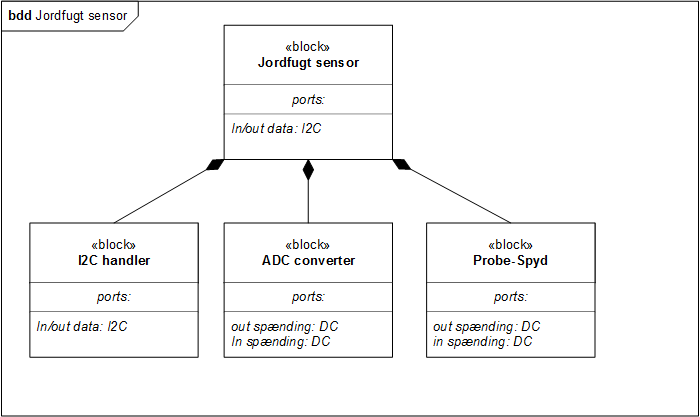
\includegraphics[width=0.82\textwidth]{Systemarkitektur/Sensor_jordfugtighed/JordFugt_probe_BDD.png}
	\label{fig:pH-sensor BDD}
	\caption{Block Definition Diagram af pH-sensor}
\end{figure}



\subsection{pH-sensor IBD}

\begin{figure}[H]
	\centering
	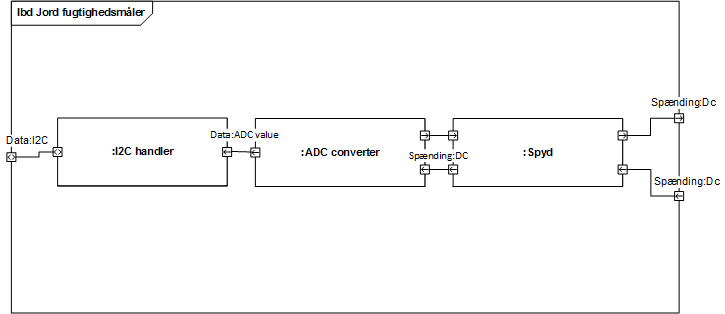
\includegraphics[width=0.82\textwidth]{Systemarkitektur/Sensor_jordfugtighed/JordFugt_probe_IBD.png}
	\label{fig:pH-sensor IBD}
	\caption{Internal Block Diagram af pH-sensor}
\end{figure}